\chapter{Laboratorium 1}
\label{cha:Lab001}
\makeatletter


% *********************************************************************
% w poniższej metryczce należy uzupełnić informacje o:
% - temacie ćwiczenia
% - numer ćwiczenia
% - numer grupy laboratoryjnej
% - numer zespołu
% - datę wykonania ćwiczenia oraz oddania ćwiczenia.
% *********************************************************************

\begin{table}[H]
    \centering
    \renewcommand{\tabularxcolumn}[1]{m{#1}}  % Dostosowanie kolumny do zawartości
    \newcolumntype{C}{>{\centering\arraybackslash}X}
    \begin{tabularx}{\linewidth}{|C|C|}
        \hline
        \multicolumn{2}{|c|}{\makecell{\textbf{\Large{Biometryczne Systemy Zabezpieczeń}} \\ \textbf{Ćwiczenia Laboratoryjne}}} \\ \hline
        \multicolumn{1}{|l|}{Temat}                    &              WPROWADZENIE DO BIBLIOTEKI MATLAB IMAGE PROCESSING ORAZ HISTOGRAMOWE METODY SEGMENTACJI OBRAZÓW.             \\ \hline
        \multicolumn{1}{|l|}{Ćwiczenie nr:}                    &      01                   \\ \hline
        \multicolumn{1}{|l|}{Autorzy:}                         &   \@author                              \\ \hline
        \multicolumn{1}{|l|}{Grupa laboratoryjna}                       &       02               \\ \hline
        \multicolumn{1}{|l|}{Zespół nr. }                       &    XX                  \\ \hline
        \multicolumn{1}{|l|}{Data wykonana ćwiczenia}         &  23.04.2025     \\ \hline
        \multicolumn{1}{|l|}{Data oddania ćwiczenia  }         &   13.05.2025     \\ \hline
    \end{tabularx}
\end{table}


\section{Cel ćwiczenia}

Celem laboratorium jest zapoznanie się z podstawowymi funkcjami biblioteki Image Processing Toolbox w MATLAB-ie oraz zastosowanie metod segmentacji obrazów opartych na analizie histogramu. Należy zapoznać się z materiałami i przykładami zawartymi w niniejszych materiałach oraz zaproponować rozwiązania dla zadań do samodzielnego rozwiązania. Rozwiązania należy umieścić w sprawozdaniu, zgodnie z wymaganiami.

\section{Wstęp teoretyczny}
Histogram obrazu to funkcja przedstawiająca rozkład wartości pikseli w obrazie. Może być wykorzystywany do:
\begin{itemize}
	\item Poprawy kontrastu obrazu (rozciąganie histogramu, wyrównywanie histogramu),
	\item Segmentacji obrazu na podstawie progów jasności (np. metoda Otsu),
	\item Analizy jakości obrazu, w tym identyfikacji prześwietlonych lub niedoświetlonych obszarów.
\end{itemize}

Histogram w obrazie monochromatycznym można obliczyć za pomocą funkcji $h(k)$, określającej liczbę pikseli o poziomie jasności $k$:
\begin{equation}
	h(k) = \sum_{(x,y) \in \Omega} \delta(I(x,y) - k),
\end{equation}
gdzie $\delta$ to funkcja Kroneckera, a $\Omega$ oznacza zbiór pikseli w obrazie.

\section{Opis wykorzystywanego oprogramowania i narzędzi}
Do przeprowadzenia eksperymentu wykorzystano środowisko MATLAB oraz bibliotekę Image Processing Toolbox. Kluczowe funkcje wykorzystane w analizie to:
\begin{itemize}
	\item \texttt{imhist} - obliczanie histogramu obrazu,
	\item \texttt{imadjust} - rozciąganie histogramu,
	\item \texttt{histeq} - wyrównywanie histogramu,
	\item \texttt{graythresh} oraz \texttt{imbinarize} - segmentacja metodą Otsu.
\end{itemize}

\section{Zadania do wykonania samodzielnego}

\subsection{Zadanie 1}

\subsubsection{Treść}
\textbf{Konwersja obrazu na różne formaty przy użyciu MATLAB i Image Processing Toolbox:}

Użyj funkcji dostępnych w bibliotece IPT w MATLAB-ie do przekształcenia obrazu. Na Rys. 9
przedstawiono schemat przepływu i konwersji różnych typów obrazów w MATLAB-ie,
z wykorzystaniem funkcji dostępnych w IPT.

\subsubsection{Pytania do analizy}

\begin{itemize}
	\item Jak zmienia się zakres wartości pikseli w kolejnych przekształceniach?
	
	\begin{itemize}
		\item RGB: 3 kanały (R, G, B), każdy z zakresem [0, 255]
		\item Monochromatyczny (gray): pojedynczy kanał, zakres [0, 255]
		\item Binarny: dwa poziomy – 0 (czarny) i 1 (biały)
		\item Indeksowany: każdy piksel to indeks w tablicy kolorów (zazwyczaj 0–255 przy 256 kolorach)
	\end{itemize}

	\item Jaka jest różnica w zajmowanej pamięci między różnymi formatami obrazów?

	\begin{itemize}
		\item \textbf{RGB}: największy rozmiar – 3 bajty na piksel (8 bitów × 3 kanały).
		\item \textbf{Gray}: 1 bajt na piksel.
		\item \textbf{Binarny}: 1 bit na piksel (oszczędność miejsca).
		\item \textbf{Indeksowany}: 1 bajt na piksel + osobna tablica kolorów (colormap).
	\end{itemize}

	\item Jakie mogą być zastosowania obrazów indeksowanych i binarnych w praktyce?

	\begin{itemize}
		\item Indeksowane:
		
		\begin{itemize}
			\item kompresja obrazów do GIF.
			\item aplikacje z ograniczoną paletą barw (np. grafika retro, przeglądarki).
		\end{itemize}
		
		\item Binarne:
		
		\begin{itemize}
			\item analiza obiektów (segmentacja, maski).
			\item OCR (rozpoznawanie tekstu).
			\item wykrywanie krawędzi, konturów.
		\end{itemize}
	\end{itemize}

\end{itemize}

\subsubsection{Przykładowy program}
\lstinputlisting[style= matlabStyle, caption= Wczytanie obrazu i stworzenie konwersji, label=Lab001_l1]{src/Lab001/zadanie1.m}

\subsubsection{Obrazy}
\begin{figure}[H]
	\centering
	\begin{subfigure}[t]{0.45\linewidth}
		\centering
		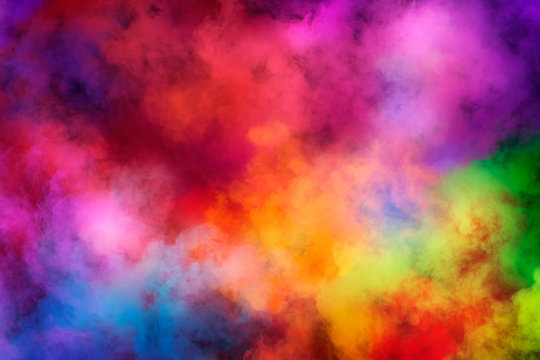
\includegraphics[width=\linewidth]{src/Lab001/zadanie1images/obraz_rgb.png}
		\caption{Obraz RGB}
		\label{fig:rgb}
	\end{subfigure}
	\hfill
	\begin{subfigure}[t]{0.45\linewidth}
		\centering
		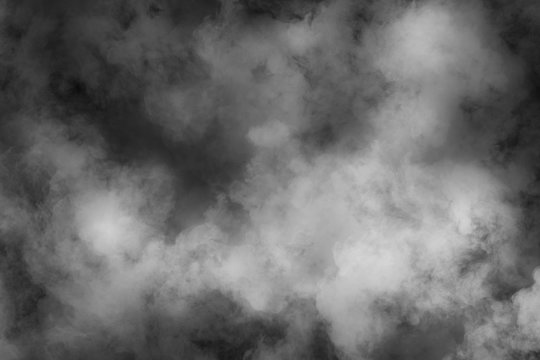
\includegraphics[width=\linewidth]{src/Lab001/zadanie1images/obraz_szary.png}
		\caption{Obraz szary}
		\label{fig:gray}
	\end{subfigure}
	
	\begin{subfigure}[t]{0.45\linewidth}
		\centering
		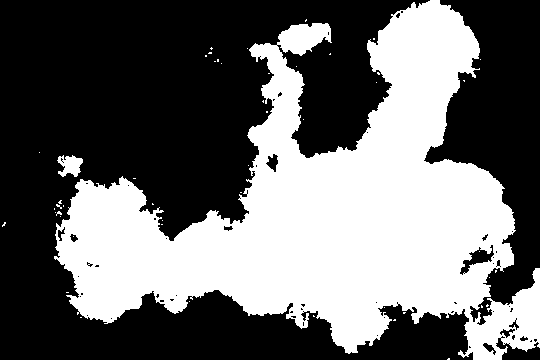
\includegraphics[width=\linewidth]{src/Lab001/zadanie1images/obraz_binarny.png}
		\caption{Obraz binarny}
		\label{fig:binary}
	\end{subfigure}
	\hfill
	\begin{subfigure}[t]{0.45\linewidth}
		\centering
		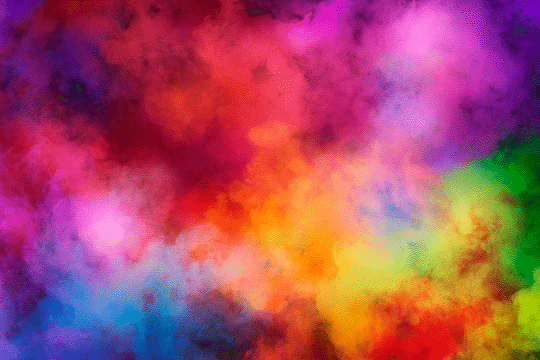
\includegraphics[width=\linewidth]{src/Lab001/zadanie1images/obraz_indeksowany.png}
		\caption{Obraz indeksowany}
		\label{fig:indexed}
	\end{subfigure}
	
	\begin{subfigure}[t]{0.45\linewidth}
		\centering
		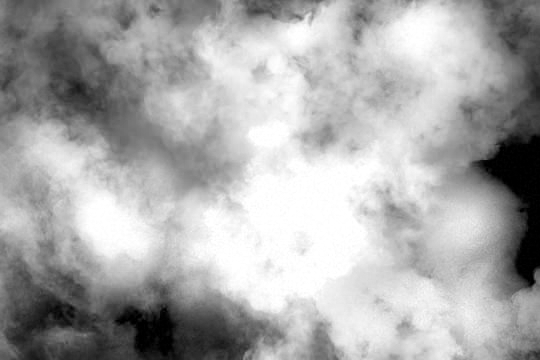
\includegraphics[width=\linewidth]{src/Lab001/zadanie1images/kanal_czerwony.png}
		\caption{Kanał czerwony}
		\label{fig:red}
	\end{subfigure}
	\hfill
	\begin{subfigure}[t]{0.45\linewidth}
		\centering
		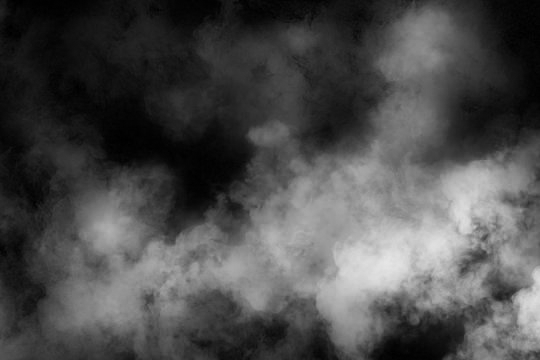
\includegraphics[width=\linewidth]{src/Lab001/zadanie1images/kanal_zielony.png}
		\caption{Kanał zielony}
		\label{fig:green}
	\end{subfigure}
	
	\begin{subfigure}[t]{0.45\linewidth}
		\centering
		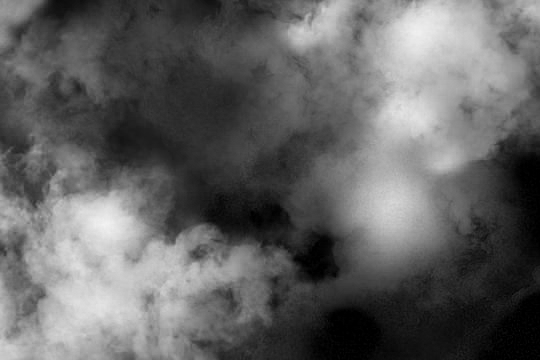
\includegraphics[width=\linewidth]{src/Lab001/zadanie1images/kanal_niebieski.png}
		\caption{Kanał niebieski}
		\label{fig:blue}
	\end{subfigure}
	
	\caption{Wizualizacja obrazów w różnych formatach i kanałach.}
	\label{fig:all_images1}
\end{figure}

\clearpage

\subsection{Zadanie 2}

\subsubsection{Treść}

\textbf{Zadanie 2. Histogram i operacje na histogramie.}

W Matlab zaproponuj program, który pozwoli na:

\begin{itemize}
	\item Wczytanie obrazu w skali szarości (imread → rgb2gray jeśli potrzeba).
	\item Obliczenie i wyświetlenie histogramu obrazu (imhist).
	\item Wykonaj rozciąganie histogramu (imadjust + stretchlim) i porównaj obraz przed i po operacji.
	\item Wykonaj wyrównanie histogramu (histeq) i porównaj wynik z oryginalnym obrazem oraz z histogramem rozciągniętym.
	\item Wyświetl histogramy wszystkich przekształconych obrazów.
\end{itemize}

\subsubsection{Przykładowy program}
\lstinputlisting[style= matlabStyle, caption= Wczytanie obrazu i przetwarzanie obrazu histogramami, label=Lab001_l2]{src/Lab001/zadanie2.m}
\clearpage

\subsubsection{Obrazy}

\begin{figure}[H]
	\begin{subfigure}[t]{0.45\linewidth}
		\centering
		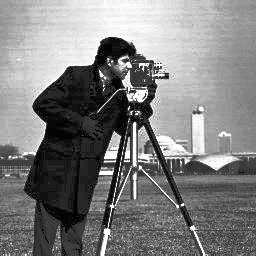
\includegraphics[width=\linewidth]{src/Lab001/zadanie2images/obraz_equalized.png}
		\caption{Obraz wyrównany}
		\label{fig:equ}
	\end{subfigure}
	\hfill
	\begin{subfigure}[t]{0.45\linewidth}
		\centering
		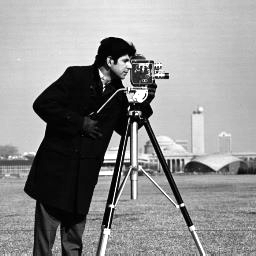
\includegraphics[width=\linewidth]{src/Lab001/zadanie2images/obraz_stretched.png}
		\caption{Obraz rozciągnięty}
		\label{fig:stretched}
	\end{subfigure}
		
	\caption{Wizualizacja rozciągania i wyrównywania obrazów}
	\label{fig:all_images2} 
\end{figure}

\subsubsection{Pytania do analizy}

\begin{itemize}
	\item Jaka jest różnica między rozciąganiem a wyrównywaniem histogramu?
	
	\begin{itemize}
		\item Rozciąganie (stretching): zmienia zakres jasności, przekształcając piksele tak, by rozciągnąć istniejący histogram do pełnego zakresu (np. 0–255).
		\item Wyrównywanie (equalization): zmienia rozkład jasności, aby histogram był możliwie równomierny – poprawiając kontrast globalnie.
	\end{itemize}
	
	\item Która metoda daje lepsze wyniki poprawy kontrastu?
	
	\begin{itemize}
		\item Dla obrazów o niskim kontraście — wyrównanie często działa lepiej.
		\item Dla obrazów z dobrze rozłożonymi poziomami jasności — rozciąganie może być wystarczające i mniej inwazyjne.
	\end{itemize}
	
	\item Jakie są potencjalne zastosowania tych technik?
	\begin{itemize}
		\item Poprawa jakości obrazów w:
		\begin{itemize}
			\item medycynie (np. obrazowanie rentgenowskie),
			\item nadzorze wizyjnym (monitoring),
			\item przetwarzaniu zdjęć satelitarnych,
			\item OCR (rozpoznawanie tekstu),	
			\item automatycznej analizy obrazów przemysłowych.
		\end{itemize}
	\end{itemize}
\end{itemize}

\clearpage

\subsection{Zadanie 3}

\subsubsection{Treść}
\textbf{Zadanie 3. Segmentacja obrazu na podstawie histogramu.}

W Matlab zaproponuj program, który pozwoli na:

\begin{itemize}
	\item Wczytanie obrazu w skali szarości.
	\item Obliczenie histogramu obrazu (imhist) i znalezienie potencjalnego progu segmentacji.
	\item Przeprowadź ręczną segmentację obrazu, stosując różne wartości progowe (BW = I > threshold).
	\item Zastosuj automatyczną segmentację metodą Otsu (graythresh + imbinarize).
	\item Porównaj efekty różnych progowań, wyświetlając wyniki obok siebie.
\end{itemize}

\subsubsection{Przykładowy program}

\lstinputlisting[style= matlabStyle, caption= Wczytanie obrazu i segmentacja na podstawie histogramu, label=Lab001_l3]{src/Lab001/zadanie3.m}
\clearpage

\subsubsection{Obrazy}

\begin{figure}[H]
	\begin{subfigure}[t]{0.45\linewidth}
		\centering
		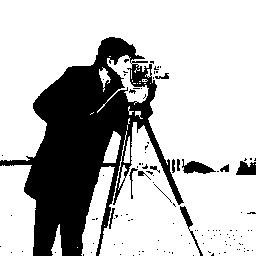
\includegraphics[width=\linewidth]{src/Lab001/zadanie3images/progowanie_80.png}
		\caption{Progowanie 80}
		\label{fig:prog80}
	\end{subfigure}
	\hfill
	\begin{subfigure}[t]{0.45\linewidth}
		\centering
		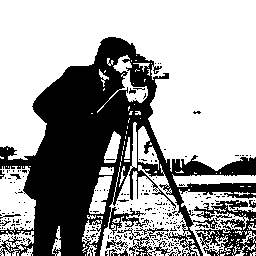
\includegraphics[width=\linewidth]{src/Lab001/zadanie3images/progowanie_120.png}
		\caption{Progowanie 120}
		\label{fig:prog120}
	\end{subfigure}
	
	\begin{subfigure}[t]{0.45\linewidth}
		\centering
		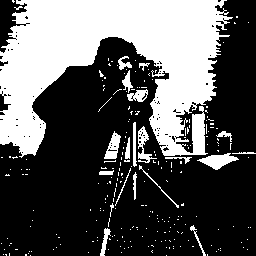
\includegraphics[width=\linewidth]{src/Lab001/zadanie3images/progowanie_160.png}
		\caption{Progowanie 160}
		\label{fig:prog160}
	\end{subfigure}
	\hfill
	\begin{subfigure}[t]{0.45\linewidth}
		\centering
		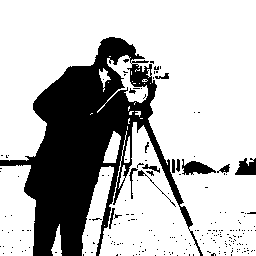
\includegraphics[width=\linewidth]{src/Lab001/zadanie3images/segmentacja_otsu.png}
		\caption{Segmentacja Otsu}
		\label{fig:sem_otsu}
	\end{subfigure}
	
	\caption{Operacje segmentowanie progowaniem oraz otsu.}
	\label{fig:all_images3} 
\end{figure}

\subsubsection{Pytania do analizy}

\begin{itemize}
	\item Jak dobrać optymalny próg segmentacji dla różnych obrazów?
	\begin{itemize}
		\item \textbf{Ręcznie}: na podstawie histogramu – szukamy wyraźnych "dolinek" (oddzielenie klas).
		\item \textbf{Automatycznie}: np. metoda Otsu – optymalizuje podział na dwie klasy o minimalnej wariancji wewnątrzklasowej.
	\end{itemize}
	
	\item Kiedy metoda Otsu jest skuteczniejsza niż segmentacja ręczna?
	\begin{itemize}
		\item Gdy histogram jest \textbf{dwumodalny} (dwa główne zbiory pikseli – tło i obiekt).
		\item Gdy chcemy \textbf{zautomatyzować} segmentację wielu obrazów bez ręcznego ustawiania progów.
		\item Gdy nie mamy wiedzy o zawartości obrazu i chcemy uzyskać ogólnie dobrą separację.
	\end{itemize}
	\clearpage
	
	\item Jakie mogą być praktyczne zastosowania binaryzacji?
	\begin{itemize}
		\item Detekcja i zliczanie obiektów (np. komórek w mikroskopii).
		\item OCR (rozpoznawanie tekstu).
		\item Analiza konturów i kształtów.
		\item Przemysł: detekcja defektów, systemy wizyjne.
		\item Monitoring: wykrywanie ruchu, segmentacja obiektów.
	\end{itemize}
\end{itemize}

\subsection{Zadanie 4}

\subsubsection{Treść}

\textbf{Zadania 4: Detekcja obiektów na obrazie binarnym.}

W Matlab zaproponuj program, który pozwoli na:

\begin{itemize}
	\item Wykonasz segmentację obrazu metodą Otsu i uzyskaj obraz binarny.
	\item Zidentyfikuj obiekty na obrazie binarnym za pomocą funkcji bwlabel lub regionprops.
	\item Wyznacz podstawowe właściwości wykrytych obiektów (np. powierzchnię, obwód).
	\item Narysuj prostokątne obramowania wokół wykrytych obiektów (rectangle).
	\item Zwizualizuj oryginalny obraz z nałożonymi obramowaniami.
\end{itemize}

\subsubsection{Przykładowy program}

\lstinputlisting[style= matlabStyle, caption= Wczytanie obrazu i dokonanie detekcji obiektów na obrazie, label=Lab001_l4]{src/Lab001/zadanie4.m}

\subsubsection{Obrazy}

\begin{figure}[H]
	\centering
	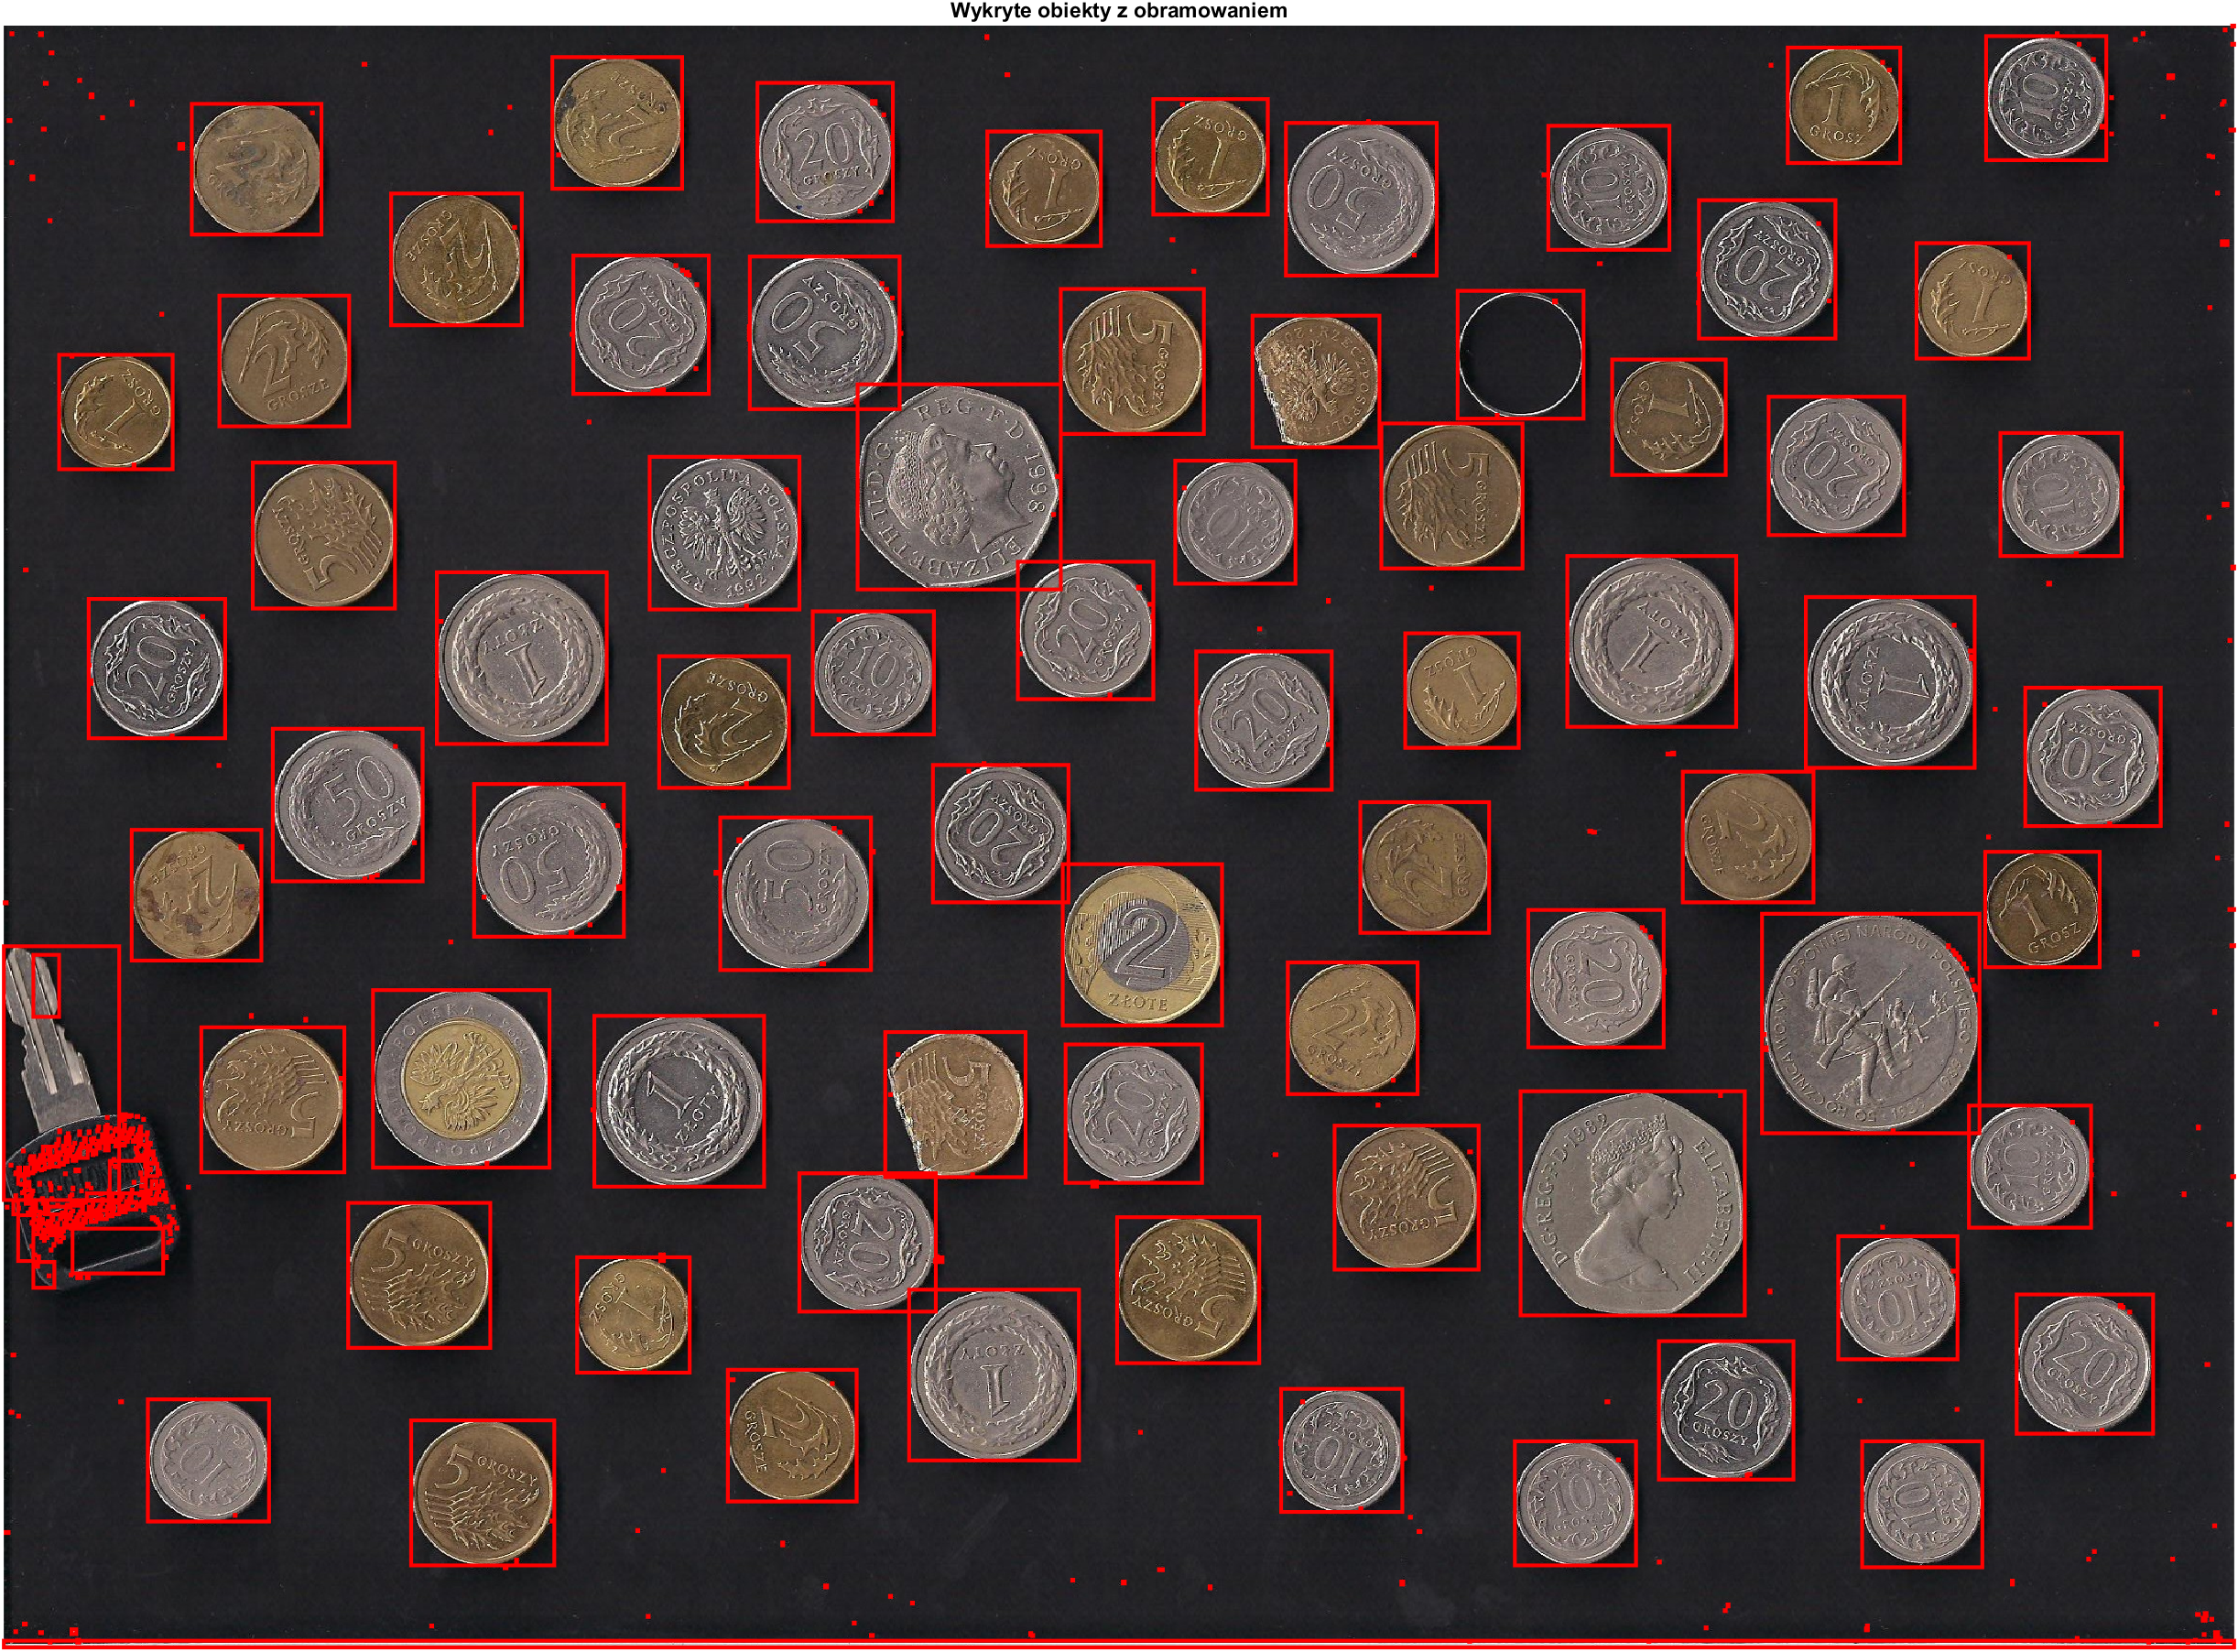
\includegraphics[width=0.7\linewidth]{src/Lab001/zadanie4images/obiekty_z_obramowaniem.png}\\
	\caption{Detekcja obiektów na obrazie.\label{fig:all_images4}}
\end{figure}

\subsubsection{Pytania do analizy}

\begin{enumerate}
	\item Jakie problemy mogą wystąpić przy detekcji obiektów w zależności od jakości segmentacji?
	\begin{itemize}
		\item Zbyt niska jakość segmentacji może prowadzić do:
		\begin{itemize}
			\item scalania sąsiadujących obiektów w jeden,
			\item pocięcia jednego obiektu na kilka części,
			\item pomijania obiektów o słabym kontraście,
			\item szumu – detekcji fałszywych obiektów.
		\end{itemize}
	\end{itemize}
	
	\item Jak można poprawić dokładność detekcji?
	\begin{itemize}
		\item Filtracja obrazu przed segmentacją (np. medfilt2, imgaussfilt).
		\item Morfologia: imopen, imclose, bwareaopen – usuwa drobne obiekty/szumy.
		\item Dostosowanie progu segmentacji ręcznie lub przez adaptacyjną binaryzację (adaptthresh).
		\item Użycie maski ROI lub filtrowanie po właściwościach (Area, Eccentricity, itp.).
	\end{itemize}
	
	\item Jakie są praktyczne zastosowania tej metody?
	\begin{itemize}
		\item \textbf{Biomedycyna}: zliczanie komórek, wykrywanie struktur w mikroskopii.
		\item \textbf{Przemysł}: kontrola jakości (np. wykrywanie wad, pomiar kształtu).
		\item \textbf{Robotyka/Widzenie maszynowe}: identyfikacja i lokalizacja obiektów.
		\item \textbf{Bezpieczeństwo}: wykrywanie tablic rejestracyjnych, ludzi, ruchu.
	\end{itemize}
\end{enumerate}

\subsection{Zadanie 5}

\subsubsection{Treść}

\textbf{Zadanie 5. Segmentacja wieloprogowa}

W Matlab zaproponuj program, który pozwoli na:

\begin{itemize}
	\item Wczytasz obraz w skali szarości.
	\item Obliczysz histogram obrazu i znajdźiesz dwa optymalne progi metodą Otsu (multithresh).
	\item Utwórz obraz segmentowany na trzy klasy (imquantize).
	\item Zwizualizuj wynik segmentacji z użyciem różnych kolorów (label2rgb).
	\item Porównaj segmentację wieloprogową z binaryzacją jednokryterialną.
\end{itemize}

\subsubsection{Przykładowy program}

\lstinputlisting[style= matlabStyle, caption= Wczytanie obrazu i dokonanie detekcji obiektów na obrazie, label=Lab001_l5]{src/Lab001/zadanie5.m}


\subsubsection{Obrazy}

\begin{figure}[H]
	\begin{subfigure}[t]{0.45\linewidth}
		\centering
		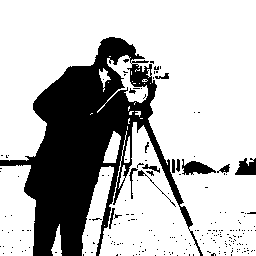
\includegraphics[width=\linewidth]{src/Lab001/zadanie5images/binaryzacja_otsu.png}
		\caption{Progowanie 80}
		\label{fig:bin_otsu}
	\end{subfigure}
	\hfill
	\begin{subfigure}[t]{0.45\linewidth}
		\centering
		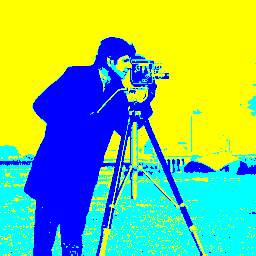
\includegraphics[width=\linewidth]{src/Lab001/zadanie5images/segmentacja_wieloprogowa.png}
		\caption{Progowanie 120}
		\label{fig:wiel_pr}
	\end{subfigure}
	
	\caption{Operacje segmentowanie wieloprogowego.}
	\label{fig:all_images5} 
\end{figure}

\subsubsection{Pytania do analizy}

\begin{enumerate}
	\item W jakich przypadkach segmentacja wieloprogowa daje lepsze wyniki niż binaryzacja?
	\begin{itemize}
		\item Gdy obraz zawiera \textbf{więcej niż dwa poziomy jasności} reprezentujące różne obiekty lub tło (np. tło, cień, obiekt).
		\item Przy obrazach z \textbf{wieloma klasami intensywności} – np. zdjęcia medyczne, zdjęcia z mikroskopu, obrazy satelitarne.
	\end{itemize}
	
	\item Jakie są ograniczenia segmentacji wieloprogowej?
	\begin{itemize}
		\item \textbf{Wymaga wiedzy} o liczbie klas (ile progów wyznaczyć).
		\item \textbf{Czasochłonna} przy większej liczbie progów lub dużych obrazach.
		\item Czasem nie sprawdza się przy słabym kontraście lub zaszumionym obrazie – klasy mogą się zlewać.
	\end{itemize}
	
	\item Jak można poprawić jakość segmentacji?
	\begin{itemize}
		\item \textbf{Filtracja} przed segmentacją (imgaussfilt, medfilt2).
		\item \textbf{Użycie morfologii} po segmentacji (imopen, imclose, bwareaopen).
		\item Dobór progów ręcznie lub przez adaptacyjne metody (adaptthresh).
		\item W połączeniu z analizą cech (regionprops) można odfiltrować obiekty niepasujące do oczekiwań.
	\end{itemize}
\end{enumerate}

\section{Wnioski}
Na podstawie przeprowadzonych eksperymentów można stwierdzić, że:
\begin{itemize}
    \item Histogram jest przydatnym narzędziem w analizie jakości obrazu biometrycznego.
    \item Wyrównanie histogramu poprawia kontrast i może zwiększać czytelność obrazu.
    \item Segmentacja oparta na histogramie, w szczególności metoda Otsu, pozwala na skuteczne wydzielenie istotnych cech obrazu.
\end{itemize}

